\section{Personal Goals}
\label{sec:personal}
\lhead{\thesection \space Personal Goals}

As mentioned in the introduction, the author defines a set of personal goals that they want to reach in order to advance their skills as mentioned in \textit{\ref{sec:development} Development}. This chapter deals with specific topics and technologies that the author will work with during the course of the project that are related to the skill levels detailed in the aforementioned chapter.

\subsection{React Native}

The author especially wants to familiarize with the framework \textit{React Native}. The component-based nature of \textit{React Native} allows the author to gain skills in the usage of interactive components to gain skills in the context of User Interaction implementation. To do so, the author wants to apply the concept of \textit{React} and \textit{React Native}, to make use of existing components and frameworks and to develop components of their own.
\newline
To prove that their skill regarding this topic have improved, the author will be able to explain the core structure of \textit{React Native} as well as being able to comprehend why an interactive component behaves the way it does and how it enhanced the User experience. Furthermore, the author would like to research possibilities to test \textit{React Native} components and applications, for example by making use of frameworks such as \textit{JestJS}, \textit{Espresso}, \textit{Detox} or other means to provide test functionality or even test automation.

\subsection{Firebase \& GraphQL}

Given that the project is based on an already existing product, the author would like to be able to design software that incorporates existing components flawlessly. The project includes components utilizing Google's \textit{Firebase} and Facebook's \textit{GraphQL} to store, transfer and query information between the frontend \textit{React Native} app and a backend consisting of \textit{Firebase} and a \textit{MongoDB} database.

\begin{figure}[!ht]
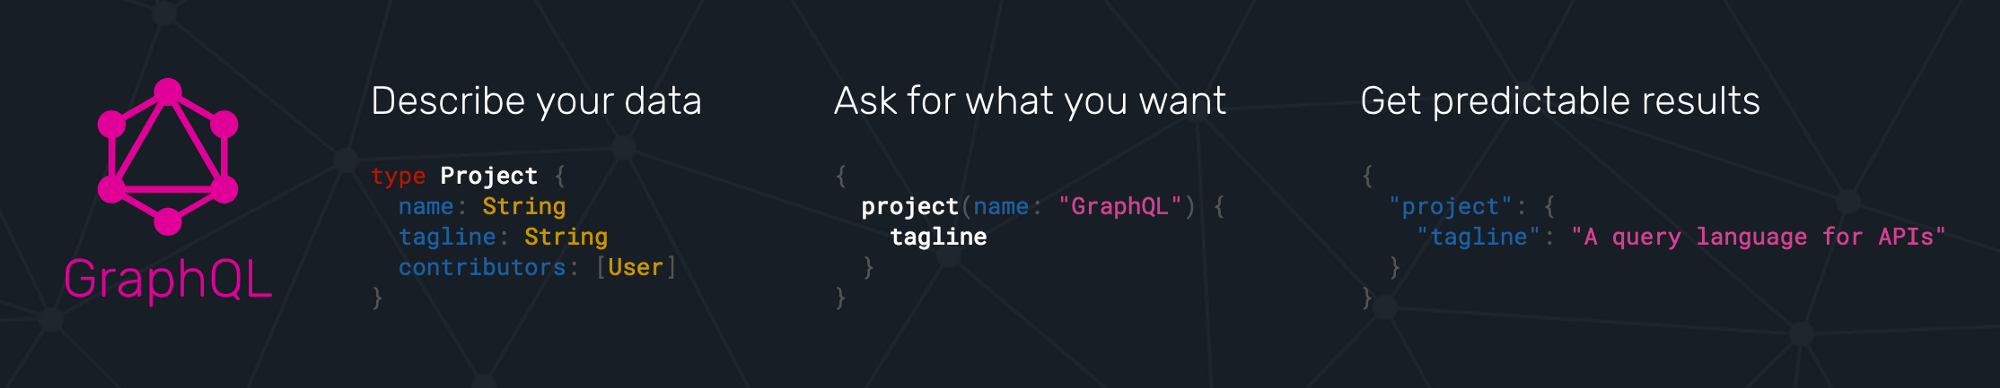
\includegraphics[width=\textwidth]{Pics/graphql.png}
\caption{GraphQL Query Definitions}
\label{fig:graphql}
\end{figure}

The author would like to design the interaction between the components to ensure a productive way to transfer information that is both easy to use and understand as well as it is offering great performance. Given that the author would like to focus on system design as well as quality assurance, the design would include a test strategy to ensure that an implementation of said design works as intended.
\newline
To prove that the author gained new skill on this topic, they will be able to comprehend why the component system of the finished product is set up as it is and how a certain level of quality is ensured by comprehending what test strategy was defined and by applying the strategy within the project.

\subsection{Management}

While not specifically related to any of the learning goals mentioned in \textit{\ref{sec:development} Development}, the author would like to familiarize with Atlassian's \textit{Jira}, a project tracking software that will be utilized over the course of the project. It is a goal to gain skills in how to use the software as well as to comprehend how the software can enhance agile software development frameworks such as \textit{Scrum}, by providing boards and other tracking method to keep track of sprints, tasks, issues and the development backlog.

\begin{figure}[!ht]
\begin{center}

\includegraphics[width=0.45\textwidth]{Pics/Jira.png}
\end{center}
\caption{Logo of Atlassian's \textit{Jira}}
\label{fig:jira}
\end{figure}

The goal of the author would be to use \textit{Jira} in a productive way to ensure an error resistant project course and smooth communication with other project members. To prove that the author gained skills in using \textit{Jira}, they will be able to apply usage of \textit{Jira} in the project and to comprehend how \textit{Jira} was utilized during the project and why they think it is a good or maybe not so good idea to use it as a project tracking software.